\documentclass[a4paper, 12pt]{article} 
\usepackage[top=2cm, bottom=2cm, left=2.5cm, right=2.5cm]{geometry}
\usepackage[utf8]{inputenc}
\usepackage{amsmath, amsfonts, amssymb}
\usepackage{graphicx} %pacote para inserir figuras
\usepackage{float} %força posicionamento da figura - para usar: subtituir [htb] por[H]
\usepackage[brazil]{babel} %força latex a escrever figura e não figure



\begin{document}


\begin{table}[htb] %para colocar numerações na tabela
	\centering %centraliza a tabela :D
	\begin{tabular}{|c|c|} %indicamos o numero de colunas com alinhamentos lrc ou p{8cm} , |==borda
		\hline
		coluna 1 & coluna 2 \\ \hline %separamos linhas com barra barra
		coluna 1 & coluna 2 \\ \hline %hline é a linha horizontal
		coluna 1 & coluna 2 \\ \hline
	\end{tabular}
	\caption{tabela legenda numerada}	
	\label{index-tabela1}	%usar \ref{index-tabela1}} para referir-se à essa tabela
\end{table}

a tabela \ref{index-tabela1} é muito legal!


\section{Veja um cabeçalho para uma tabela:}

\begin{center}
	\begin{tabular}{cp{10cm}}
	\hline
		\begin{tabular}{c}
			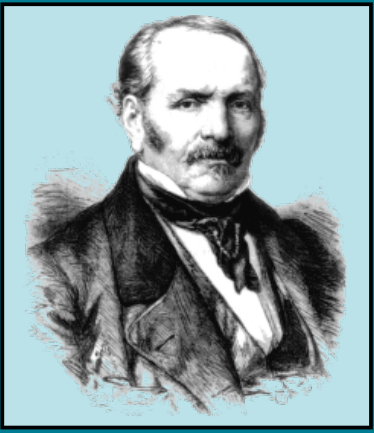
\includegraphics[scale=0.1]{img/kardec.png}				
		\end{tabular} & %aqui começa segunda coluna
		\begin{tabular}{l}
		latex é um negocio doido mano \\
		to aprendendo e curtindo \\
		legal \\
		
		\end{tabular}
	
	\end{tabular}
\end{center}
	

\end{document}
